
% ==================================================
%	Theorie
% ==================================================

\section{Theorie}
	In der Quantentheorie können die Elektronen einer Atomhülle eines
	Atoms nur abzählbar viele Zustände annehmen, die durch die
	Quantenzahlen
	\begin{itemize}
	\item Elektronenspin $S$, für Elektronen ist $S=\nicefrac{1}{2}$
	\item Kernspin $I$, für $\Rb95$ ist $I=\nicefrac{5}{2}$
	\item Bahndrehimpuls $L\geq 0$
	\item Drehimpuls der Elektronenhülle $J\in\{ |S-L|,|S-L|+1,
	\ldots , S+L-1, S+L \}$
	\item Gesamtdrehimpuls $F\in \{|J-I|,|J-I|+1,\ldots , J+I-1, J+I\}$
	\end{itemize}
	charakterisiert werden.
	Zusätzlich werden die Quantenzahlen $m_S$, $m_L \in
	(-S\text{ bzw. }-L,
	S\text{ bzw. }L) \cap \mathbb{Z}$ und $m_F\in (-F,F)\cap
	\mathbb{Z}$ eingeführt, sodass
	ein eindeutiger
	Elektronenzustand $|s,l,j\rangle$ definiert werden kann. Im
	allgemeinen können die Zustände jedoch entartet sein, d.h.
	verschiedenen Zuständen haben die gleiche Energie\footnote{Im
	Folgenden ist ein Energieniveau die Menge der $g$ Zustände selber
	Energie. Wird verschiedenen Zuständen die gleiche Energie
	zugeordnet, so spricht man von \text{Entartung}.}.
	Aufgrund des Pauli-Prinzips kann
	jeder Elektronenzustand nur einfach besetzt werden, sodass
	Zustände niedriger Energie "`aufgefüllt"' sind, da hier
	thermische Prozesse keine Rolle spielen. Für
	zwei nicht aufgefüllte Energieniveaus $1$ und $2$ mit Energien
	$W_1$, $W_2$
	und 	Besetzungszahlen $N_1$, $N_2$ gilt dagegen die Boltzmannsche
	Gleichung \cite{Praktikum}
	\begin{equation}
		\frac{N_2}{N_1} =
		\frac{g_2}{g_1}\frac{e^\nicefrac{-W_2}{k_\text{B} T}}{
		e^\nicefrac{-W_1}{k_\text{B} T}}
		 \label{eq:Boltzmann} .
	\end{equation}
	Die magnetischen Momente werden mit dem Bohrschen Magneton
	$\upmu_\text{B}$ über
	\begin{align}
		|\vec{\mu}_S| & = g_S \upmu_\text{B} \sqrt{ S(S +1)} \\
		|\vec{\mu}_L| & = \upmu_\text{B} \sqrt{ L(L +1)} \\
		|\vec{\mu}_J| & =g_J \upmu_\text{B} \sqrt{ J(J +1)}
	\end{align}
	definiert, wobei $g_S$ und $g_J$ die Lande-Faktoren des Spins
	bzw. des Drehimpulses der Elektronenhülle sind.

	Im Experiment können die energetisch verschiedenen Zustände des
	Atoms mit Hilfe der Elektromagnetischen Strahlung nachgewiesen
	werden, welche beim Übergang vom energetisch höheren Zustand i zum
	energetisch niedrigeren Zustand f
	emittiert wird. Sind $W_\text{i}$ und
	$W_\text{f}$  die Energien des Anfangs- und Endniveaus, so wird
	mit dem Plankschen Wirkungsquantum $\text{h}$ durch
	\begin{equation}
		\text{h} \nu = W_\text{f}- W_\text{i} \label{eq:hnu}
	\end{equation}
	die Frequenz $\nu$ der emittierten Strahlung gegeben.

	Folgende Effekte beeinflussen die Energie eines Zustandes und
	führen so teilweise zur Aufhebung der Entartung.
	\begin{itemize}
		\item Die LS-Kopplung beschreibt die Wechselwirkung zwischen
			Spin $S$ und Bahndrehimpuls $L$ der Elektronenhülle. Dadurch
			wird
			die Entartung in $L$ aufgehoben. Dies liefert einen
			Beitrag zur \textit{Feinstruktur} des Spektrums.
            Für den Land\'{e}-Faktor $g_J$ gilt
            \begin{equation}
              g_J = \frac{3.0023 J(J+1) + 1.0023 \qty[S(S+1) - L(L+1)]}{2J(J+1)}~.
              \label{eq:g_J}
            \end{equation}
		\item Die Wechselwirkung zwischen dem Drehimpuls der
			Elektronenhülle $J$ und dem Kernspin $I$, durch die
			die Entartung in $F$ aufgehoben wird, wird als
			\textit{Hyperfeinstruktur} bezeichnet.
		\item Im äußeren Magnetfeld $\vec{B}$ verschiebt sich die
			Energie eines Zustandes um
            \begin{equation}
              U = \text{h} \nu = g_F \upmu_\text{B} |\vec{B}|
            \end{equation}
			diesen Effekt bezeichnet man als \textit{Zeeman-Effekt}
           \cite{Praktikum}; er hebt die Entartung in
           $m_f$ auf.
       \end{itemize}
	Für den dabei eingeführten Lande-Faktor gilt dabei
	\begin{equation}
		g_F \approx g_J \frac{F(F+1)+J(J+1)-I(I+1)}{2F(F+1)} \quad .
		\label{eq:g_F}
	\end{equation}

	Nun soll das Prinzip des Optischen Pumpens an einem hypothetischen
	Alkali-Atom, d.h. mit einem Valenzelektron, und ohne Kernspin
	erläutert werden\footnote{Für $I=0$ ist $F=J$, sodass ab
	jetzt $J$ und $m_J$ die relevanten Quantenzahlen sind.}. Wie in
	Abbildung \ref{fig:Termschema} zu sehen ist, gibt es
	\begin{figure}
		\centering
		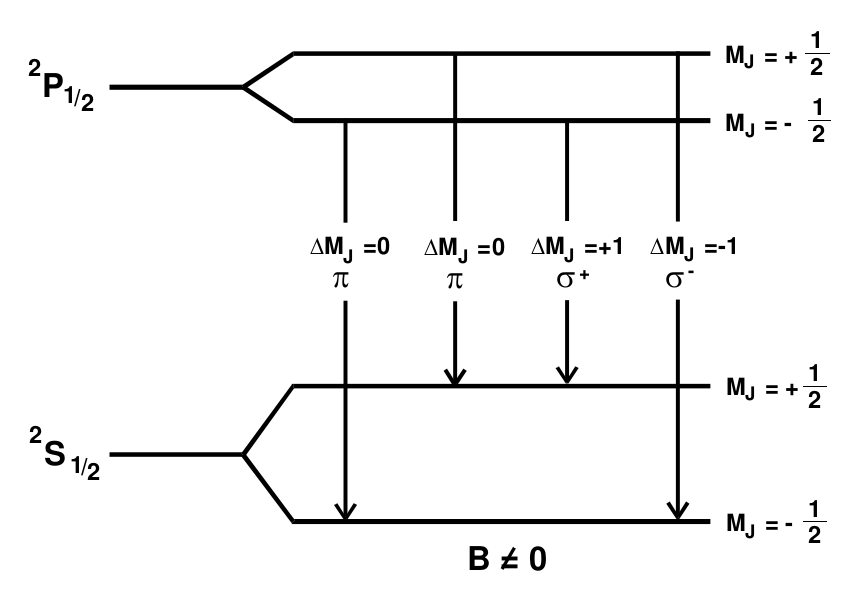
\includegraphics[scale=0.3]{bilder/termschema}
		\caption{Beispielhaftes Termschema eines Alkali-Atoms im
          äußeren Magnetfeld $|\vec{B}|$. \cite{Praktikum}}
		\label{fig:Termschema}
	\end{figure}
	zwischen dem $S_{\nicefrac12}$ (d.h. $L=0,J=\nicefrac12$) und
	$P_{\nicefrac12}$ (d.h. $L=1,J=\nicefrac12$) Energieniveau vier
	mögliche Übergänge.
	Durch Anregung mit rechtszirkular polarisierter
	Strahlung kann nun gezielt der $\sigma^+$ Übergang vom
	$S_{\nicefrac12}$ in
	ein $P_{\nicefrac12}$ hervorgerufen
	werden. Durch spontane Emission fällt das Elektron wieder auf das
	$S_{\nicefrac12}$ Niveau mit $m_J=\nicefrac12$ oder
	$m_J=-\nicefrac12$
	zurück. Durch Wiederholung dieses Vorgangs in einem viele-Atome
	System wird dadurch der Zustand $S_{\nicefrac12},m_J=\nicefrac12$
	angereichert. Effektiv ist die Transmittivität des Systems für
	diese Art der Strahlung zunächst gering, steigt jedoch, sobald
	der Zustand $S_{\nicefrac12},m_J=-\nicefrac12$ wenig bis nicht mehr besetzt
	ist.

	Durch das Anlegen eines Hochfrequenzfeldes der Frequenz $\nu$
	kommt es, falls die Zeemann-Aufspaltung
	$\text{h} }nu$ entspricht, zu induzierter Emission. Bei
	festgehaltener Frequenz $\nu$ kann nun das Magnetfeld so
	eingestellt werden, dass die Zeeman-Aufspaltung zwischen den
	zwei Niveaus genau
	\begin{equation}
		\text{h}\nu = g_J \upmu_\text{B} |\vec{B}| \label{eq:B}
	\end{equation}
	entspricht.
    Für das Magnetfeld $B$ gilt entsprechend
     \begin{equation}
       B_m = \frac{4 \uppi m_0}{e_J g_J} \nu
       \label{eq:Bm}
     \end{equation}
     mit
     \begin{equation}
       \upmu_B = \frac{e_0}{4 \uppi} \text{h}~.
     \end{equation}
     Dadurch wird das
	$m_J=-\nicefrac12$ Niveau wieder gefüllt und die Transmittivität
	nimmt ab.

	Die bisherigen Ergebnisse wurden im Grenzfall kleiner Magnetfelder
	ermittelt, sodass sie in der ersten Ordnung von $|\vec{B}|$ sind. Unter
	Berücksichtigung der zweiten Ordnung von $|\vec{B}|$ und mit Kernspin
	ergibt sich die Breit-Rabi Formel
	\begin{equation}
		U=g_F \uppmu_\text{B} |\vec{B}|+g_F^2 \upmu_\text{B}^2
		|\vec{B}|^2 \frac{1-2 m_F}{\Delta E_\text{Hy}}
		\label{eq:Breit-Rabi}
	\end{equation}
	, die den quadratischen Zeemaneffekt beschreibt, wobei $\Delta E_\text{Hy}$
	die Hyperfeinstrukturaufspaltung
	zwischen den Energieniveaus $F$ und $F+1$ darstellt.

